%\VignetteIndexEntry{ChIP-Seq Workflow Template}
%\VignetteDepends{rjson, ggplot2, limma, edgeR, GOstats, GO.db, annotate, pheatmap}
%\VignetteKeywords{compute cluster, pipeline, reports}
%\VignetteEngine{knitr::knitr}
%\VignettePackage{systemPipeR}

% Generate vignette with knitr
% R CMD Sweave --engine=knitr::knitr --pdf systemPipeChIPseq.Rnw

\documentclass{article}\usepackage[]{graphicx}\usepackage[]{color}
%% maxwidth is the original width if it is less than linewidth
%% otherwise use linewidth (to make sure the graphics do not exceed the margin)
\makeatletter
\def\maxwidth{ %
  \ifdim\Gin@nat@width>\linewidth
    \linewidth
  \else
    \Gin@nat@width
  \fi
}
\makeatother

\definecolor{fgcolor}{rgb}{0.345, 0.345, 0.345}
\newcommand{\hlnum}[1]{\textcolor[rgb]{0.686,0.059,0.569}{#1}}%
\newcommand{\hlstr}[1]{\textcolor[rgb]{0.192,0.494,0.8}{#1}}%
\newcommand{\hlcom}[1]{\textcolor[rgb]{0.678,0.584,0.686}{\textit{#1}}}%
\newcommand{\hlopt}[1]{\textcolor[rgb]{0,0,0}{#1}}%
\newcommand{\hlstd}[1]{\textcolor[rgb]{0.345,0.345,0.345}{#1}}%
\newcommand{\hlkwa}[1]{\textcolor[rgb]{0.161,0.373,0.58}{\textbf{#1}}}%
\newcommand{\hlkwb}[1]{\textcolor[rgb]{0.69,0.353,0.396}{#1}}%
\newcommand{\hlkwc}[1]{\textcolor[rgb]{0.333,0.667,0.333}{#1}}%
\newcommand{\hlkwd}[1]{\textcolor[rgb]{0.737,0.353,0.396}{\textbf{#1}}}%

\usepackage{framed}
\makeatletter
\newenvironment{kframe}{%
 \def\at@end@of@kframe{}%
 \ifinner\ifhmode%
  \def\at@end@of@kframe{\end{minipage}}%
  \begin{minipage}{\columnwidth}%
 \fi\fi%
 \def\FrameCommand##1{\hskip\@totalleftmargin \hskip-\fboxsep
 \colorbox{shadecolor}{##1}\hskip-\fboxsep
     % There is no \\@totalrightmargin, so:
     \hskip-\linewidth \hskip-\@totalleftmargin \hskip\columnwidth}%
 \MakeFramed {\advance\hsize-\width
   \@totalleftmargin\z@ \linewidth\hsize
   \@setminipage}}%
 {\par\unskip\endMakeFramed%
 \at@end@of@kframe}
\makeatother

\definecolor{shadecolor}{rgb}{.97, .97, .97}
\definecolor{messagecolor}{rgb}{0, 0, 0}
\definecolor{warningcolor}{rgb}{1, 0, 1}
\definecolor{errorcolor}{rgb}{1, 0, 0}
\newenvironment{knitrout}{}{} % an empty environment to be redefined in TeX

\usepackage{alltt}
%<<style, eval=TRUE, echo=FALSE, results=tex>>=
%BiocStyle::latex(use.unsrturl=FALSE)
%@
\RequirePackage{/usr/local/lib/R/site-library/BiocStyle/resources/tex/Bioconductor}



\usepackage[authoryear,round]{natbib}
\bibliographystyle{plainnat}
\def\bibsection{\section{References}}

\usepackage{graphicx}
\usepackage{color}
\usepackage{hyperref}
\usepackage{url}
\usepackage{float}

%\newcommand{\comment}[1]{}
%\newcommand{\Rfunction}[1]{{\texttt{#1}}}
%\newcommand{\Robject}[1]{{\texttt{#1}}}
%\newcommand{\Rpackage}[1]{{\textit{#1}}}
%\newcommand{\Rmethod}[1]{{\texttt{#1}}}
\newcommand{\Rfunarg}[1]{{\texttt{#1}}}
%\newcommand{\Rclass}[1]{{\textit{#1}}}
	
% Define header and footer area with fandyhdr package (see: http://www.ctan.org/tex-archive/macros/latex/contrib/fancyhdr/fancyhdr.pdf)
\usepackage{fancyhdr}
\pagestyle{fancy}
\fancyhead{}
\fancyfoot{}
\rhead{\nouppercase{\leftmark}}
\lhead{\textit{systemPipeR ChIP-Seq Workflow}}
\rfoot{\thepage}
\IfFileExists{upquote.sty}{\usepackage{upquote}}{}
\begin{document}



\title{ChIP-Seq workflow template: Some Descriptive Title}
\author{Project ID: ChIPseq\_PI\_Name\_Organism\_Jun2015 \\
	Project PI: First Last (first.last@inst.edu)\\
        Author of Report: First Last (first.last@inst.edu)}
\maketitle

\tableofcontents

\section{Introduction}
\subsection{Background and objectives}
This report describes the analysis of several ChIP-Seq experiments studying the DNA binding patterns of the transcriptions factors ... from \textit{organism} .... 

\subsection{Experimental design}
Typically, users want to specify here all information relevant for the analysis of their NGS study. This includes detailed descriptions of FASTQ files, experimental design, reference genome, gene annotations, etc.  

\section{Load workflow environment}

\subsection{Load packages and sample data}
The \Rpackage{systemPipeR} package needs to be loaded to perform the analysis steps shown in this report \citep{Girke2014-oy}. 
\begin{knitrout}
\definecolor{shadecolor}{rgb}{0.969, 0.969, 0.969}\color{fgcolor}\begin{kframe}
\begin{alltt}
\hlkwd{library}\hlstd{(systemPipeR)}
\end{alltt}
\end{kframe}
\end{knitrout}

Load workflow environment with sample data into your current working directory. The sample data are described  \href{http://www.bioconductor.org/packages/devel/bioc/vignettes/systemPipeR/inst/doc/systemPipeR.html#load-sample-data-and-workflow-templates}{\textcolor{blue}{here}}.
\begin{knitrout}
\definecolor{shadecolor}{rgb}{0.969, 0.969, 0.969}\color{fgcolor}\begin{kframe}
\begin{alltt}
\hlkwd{library}\hlstd{(systemPipeRdata)}
\hlkwd{genWorkenvir}\hlstd{(}\hlkwc{workflow}\hlstd{=}\hlstr{"chipseq"}\hlstd{)}
\hlkwd{setwd}\hlstd{(}\hlstr{"chipseq"}\hlstd{)}
\end{alltt}
\end{kframe}
\end{knitrout}

In the workflow environments generated by \Rfunction{genWorkenvir} all data inputs are stored in a \Robject{data/} directory and all analysis results will be written to a separate \Robject{results/} directory, while the \Robject{systemPipeChIPseq.Rnw} script and the \Robject{targets} file are expected to be located in the parent directory. The R session is expected to run from this parent directory. Additional parameter files are stored under \Robject{param/}.

To work with real data, users want to organize their own data similarly and substitute all test data for their own data. To rerun an established workflow on new data, the initial \Robject{targets} file along with the corresponding FASTQ files are usually the only inputs the user needs to provide.

If applicable users can load custom functions not provided by \Rpackage{systemPipeR}. Skip this step if this is not the case.
\begin{knitrout}
\definecolor{shadecolor}{rgb}{0.969, 0.969, 0.969}\color{fgcolor}\begin{kframe}
\begin{alltt}
\hlkwd{source}\hlstd{(}\hlstr{"systemPipeChIPseq_Fct.R"}\hlstd{)}
\end{alltt}
\end{kframe}
\end{knitrout}

\subsection{Experiment definition provided by \Robject{targets} file}
The \href{run:targets_chip.txt}{\Robject{targets}} file defines all FASTQ files and sample comparisons of the analysis workflow. 
\begin{knitrout}
\definecolor{shadecolor}{rgb}{0.969, 0.969, 0.969}\color{fgcolor}\begin{kframe}
\begin{alltt}
\hlstd{targetspath} \hlkwb{<-} \hlkwd{system.file}\hlstd{(}\hlstr{"extdata"}\hlstd{,} \hlstr{"targets_chip.txt"}\hlstd{,} \hlkwc{package}\hlstd{=}\hlstr{"systemPipeR"}\hlstd{)}
\hlstd{targets} \hlkwb{<-} \hlkwd{read.delim}\hlstd{(targetspath,} \hlkwc{comment.char} \hlstd{=} \hlstr{"#"}\hlstd{)}
\hlstd{targets[}\hlnum{1}\hlopt{:}\hlnum{4}\hlstd{,}\hlopt{-}\hlkwd{c}\hlstd{(}\hlnum{5}\hlstd{,}\hlnum{6}\hlstd{)]}
\end{alltt}
\begin{verbatim}
                  FileName SampleName Factor SampleLong SampleReference
1 ./data/SRR446027_1.fastq        M1A     M1  Mock.1h.A                
2 ./data/SRR446028_1.fastq        M1B     M1  Mock.1h.B                
3 ./data/SRR446029_1.fastq        A1A     A1   Avr.1h.A             M1A
4 ./data/SRR446030_1.fastq        A1B     A1   Avr.1h.B             M1B
\end{verbatim}
\end{kframe}
\end{knitrout}

\section{Read preprocessing}
\subsection{Read quality filtering and trimming}
The following example shows how one can design a custom read preprocessing function using utilities provided by the \Rpackage{ShortRead} package, and then apply it with \Rfunction{preprocessReads} in batch mode to all FASTQ samples referenced in the corresponding \Robject{SYSargs} instance (\Robject{args} object below). More detailed information on read preprocessing is provided in \Rpackage{systemPipeR}'s main vignette.
\begin{knitrout}
\definecolor{shadecolor}{rgb}{0.969, 0.969, 0.969}\color{fgcolor}\begin{kframe}
\begin{alltt}
\hlstd{args} \hlkwb{<-} \hlkwd{systemArgs}\hlstd{(}\hlkwc{sysma}\hlstd{=}\hlstr{"param/trim.param"}\hlstd{,} \hlkwc{mytargets}\hlstd{=}\hlstr{"targets_chip.txt"}\hlstd{)}
\hlstd{filterFct} \hlkwb{<-} \hlkwa{function}\hlstd{(}\hlkwc{fq}\hlstd{,} \hlkwc{cutoff}\hlstd{=}\hlnum{20}\hlstd{,} \hlkwc{Nexceptions}\hlstd{=}\hlnum{0}\hlstd{) \{}
    \hlstd{qcount} \hlkwb{<-} \hlkwd{rowSums}\hlstd{(}\hlkwd{as}\hlstd{(}\hlkwd{quality}\hlstd{(fq),} \hlstr{"matrix"}\hlstd{)} \hlopt{<=} \hlstd{cutoff)}
    \hlstd{fq[qcount} \hlopt{<=} \hlstd{Nexceptions]} \hlcom{# Retains reads where Phred scores are >= cutoff with N exceptions}
\hlstd{\}}
\hlkwd{preprocessReads}\hlstd{(}\hlkwc{args}\hlstd{=args,} \hlkwc{Fct}\hlstd{=}\hlstr{"filterFct(fq, cutoff=20, Nexceptions=0)"}\hlstd{,} \hlkwc{batchsize}\hlstd{=}\hlnum{100000}\hlstd{)}
\hlkwd{writeTargetsout}\hlstd{(}\hlkwc{x}\hlstd{=args,} \hlkwc{file}\hlstd{=}\hlstr{"targets_chip_trim.txt"}\hlstd{,} \hlkwc{overwrite}\hlstd{=}\hlnum{TRUE}\hlstd{)}
\end{alltt}
\end{kframe}
\end{knitrout}

\subsection{FASTQ quality report}
The following \Rfunction{seeFastq} and \Rfunction{seeFastqPlot} functions generate and plot a series of
useful quality statistics for a set of FASTQ files including per cycle quality
box plots, base proportions, base-level quality trends, relative k-mer
diversity, length and occurrence distribution of reads, number of reads above
quality cutoffs and mean quality distribution. The results are written to a PDF file named 
\href{run:./results/fastqReport.pdf}{\Robject{fastqReport.pdf}}.

\begin{knitrout}
\definecolor{shadecolor}{rgb}{0.969, 0.969, 0.969}\color{fgcolor}\begin{kframe}
\begin{alltt}
\hlstd{args} \hlkwb{<-} \hlkwd{systemArgs}\hlstd{(}\hlkwc{sysma}\hlstd{=}\hlstr{"param/bowtieSE.param"}\hlstd{,} \hlkwc{mytargets}\hlstd{=}\hlstr{"targets_chip_trim.txt"}\hlstd{)}
\hlstd{fqlist} \hlkwb{<-} \hlkwd{seeFastq}\hlstd{(}\hlkwc{fastq}\hlstd{=}\hlkwd{infile1}\hlstd{(args),} \hlkwc{batchsize}\hlstd{=}\hlnum{100000}\hlstd{,} \hlkwc{klength}\hlstd{=}\hlnum{8}\hlstd{)}
\hlkwd{pdf}\hlstd{(}\hlstr{"./results/fastqReport.pdf"}\hlstd{,} \hlkwc{height}\hlstd{=}\hlnum{18}\hlstd{,} \hlkwc{width}\hlstd{=}\hlnum{4}\hlopt{*}\hlkwd{length}\hlstd{(fqlist))}
\hlkwd{seeFastqPlot}\hlstd{(fqlist)}
\hlkwd{dev.off}\hlstd{()}
\end{alltt}
\end{kframe}
\end{knitrout}
\begin{figure}[H]
  \centering
   
\includegraphics[width=18cm]{fastqReport.pdf}
   \caption{QC report for 18 FASTQ files.}
   \label{fig:fastqreport}
\end{figure}

\section{Alignments}
\subsection{Read mapping with \Rfunction{Bowtie2}}
The NGS reads of this project will be aligned with \Robject{Bowtie2} against the reference genome sequence \citep{Langmead2012-bs}. The parameter settings of the aligner are defined in the \Robject{bowtieSE.param} file. In ChIP-Seq experiments it is usually more appropriate to eliminate reads mapping to multiple locations. To achieve this, users wants to remove the argument setting '\Rfunarg{-k 50 --non-deterministic}' in the \Robject{bowtieSE.param} file.
\begin{knitrout}
\definecolor{shadecolor}{rgb}{0.969, 0.969, 0.969}\color{fgcolor}\begin{kframe}
\begin{alltt}
\hlstd{args} \hlkwb{<-} \hlkwd{systemArgs}\hlstd{(}\hlkwc{sysma}\hlstd{=}\hlstr{"param/bowtieSE.param"}\hlstd{,} \hlkwc{mytargets}\hlstd{=}\hlstr{"targets_chip_trim.txt"}\hlstd{)}
\hlkwd{sysargs}\hlstd{(args)[}\hlnum{1}\hlstd{]} \hlcom{# Command-line parameters for first FASTQ file}
\hlkwd{moduleload}\hlstd{(}\hlkwd{modules}\hlstd{(args))} \hlcom{# Skip if a module system is not used}
\hlkwd{system}\hlstd{(}\hlstr{"bowtie2-build ./data/tair10.fasta ./data/tair10.fasta"}\hlstd{)} \hlcom{# Indexes reference genome}
\hlkwd{runCommandline}\hlstd{(args)}
\hlkwd{writeTargetsout}\hlstd{(}\hlkwc{x}\hlstd{=args,} \hlkwc{file}\hlstd{=}\hlstr{"targets_bam.txt"}\hlstd{,} \hlkwc{overwrite}\hlstd{=}\hlnum{TRUE}\hlstd{)}
\end{alltt}
\end{kframe}
\end{knitrout}
Check whether all BAM files have been created
\begin{knitrout}
\definecolor{shadecolor}{rgb}{0.969, 0.969, 0.969}\color{fgcolor}\begin{kframe}
\begin{alltt}
\hlkwd{file.exists}\hlstd{(}\hlkwd{outpaths}\hlstd{(args))}
\end{alltt}
\end{kframe}
\end{knitrout}

\subsection{Read and alignment stats}
The following provides an overview of the number of reads in each sample and how many of them aligned to the reference.
\begin{knitrout}
\definecolor{shadecolor}{rgb}{0.969, 0.969, 0.969}\color{fgcolor}\begin{kframe}
\begin{alltt}
\hlstd{read_statsDF} \hlkwb{<-} \hlkwd{alignStats}\hlstd{(}\hlkwc{args}\hlstd{=args)}
\hlkwd{write.table}\hlstd{(read_statsDF,} \hlstr{"results/alignStats.xls"}\hlstd{,} \hlkwc{row.names}\hlstd{=}\hlnum{FALSE}\hlstd{,} \hlkwc{quote}\hlstd{=}\hlnum{FALSE}\hlstd{,} \hlkwc{sep}\hlstd{=}\hlstr{"\textbackslash{}t"}\hlstd{)}
\hlkwd{read.delim}\hlstd{(}\hlstr{"results/alignStats.xls"}\hlstd{)}
\end{alltt}
\end{kframe}
\end{knitrout}

\subsection{Create symbolic links for viewing BAM files in IGV}
The \Rfunction{symLink2bam} function creates symbolic links to view the BAM alignment files in a genome browser such as IGV without moving these large files to a local system. The corresponding URLs are written to a file with a path specified under \Robject{urlfile}, here \href{run:./results/IGVurl.txt}{IGVurl.txt}.
\begin{knitrout}
\definecolor{shadecolor}{rgb}{0.969, 0.969, 0.969}\color{fgcolor}\begin{kframe}
\begin{alltt}
\hlkwd{symLink2bam}\hlstd{(}\hlkwc{sysargs}\hlstd{=args,} \hlkwc{htmldir}\hlstd{=}\hlkwd{c}\hlstd{(}\hlstr{"~/.html/"}\hlstd{,} \hlstr{"somedir/"}\hlstd{),}
            \hlkwc{urlbase}\hlstd{=}\hlstr{"http://biocluster.ucr.edu/~tgirke/"}\hlstd{,}
            \hlkwc{urlfile}\hlstd{=}\hlstr{"./results/IGVurl.txt"}\hlstd{)}
\end{alltt}
\end{kframe}
\end{knitrout}

\section{Peak calling with MACS2} 
\subsection{Merge BAM files of replicates prior to peak calling}
Merging BAM files of technical and/or biological replicates can improve the sensitivity of the peak calling by increasing the depth of read coverage. The \Rfunction{mergeBamByFactor} function merges BAM files based on grouping information specified by a \Rfunction{factor}, here the \Rfunarg{Factor} column of the imported targets file. It also returns an updated \Rfunarg{SYSargs} object containing the paths to the merged BAM files as well as to any unmerged files without replicates. This step can be skipped if merging of BAM files is not desired. 
\begin{knitrout}
\definecolor{shadecolor}{rgb}{0.969, 0.969, 0.969}\color{fgcolor}\begin{kframe}
\begin{alltt}
\hlstd{args} \hlkwb{<-} \hlkwd{systemArgs}\hlstd{(}\hlkwc{sysma}\hlstd{=}\hlkwa{NULL}\hlstd{,} \hlkwc{mytargets}\hlstd{=}\hlstr{"targets_bam.txt"}\hlstd{)}
\hlstd{args_merge} \hlkwb{<-} \hlkwd{mergeBamByFactor}\hlstd{(args,} \hlkwc{overwrite}\hlstd{=}\hlnum{TRUE}\hlstd{)}
\hlkwd{writeTargetsout}\hlstd{(}\hlkwc{x}\hlstd{=args_merge,} \hlkwc{file}\hlstd{=}\hlstr{"targets_mergeBamByFactor.txt"}\hlstd{,} \hlkwc{overwrite}\hlstd{=}\hlnum{TRUE}\hlstd{)}
\end{alltt}
\end{kframe}
\end{knitrout}

\subsection{Peak calling without input/reference sample}
MACS2 can perform peak calling on ChIP-Seq data with and without input samples \citep{Zhang2008-pc}. The following performs peak calling without input on all samples specified in the corresponding \Robject{args} object. Note, due to the small size of the sample data, MACS2 needs to be run here with the '\Rfunarg{--nomodel}' setting. For real data sets, users want to remove this parameter in the corresponding \Robject{*.param} file(s).
\begin{knitrout}
\definecolor{shadecolor}{rgb}{0.969, 0.969, 0.969}\color{fgcolor}\begin{kframe}
\begin{alltt}
\hlstd{args} \hlkwb{<-} \hlkwd{systemArgs}\hlstd{(}\hlkwc{sysma}\hlstd{=}\hlstr{"param/macs2_noinput.param"}\hlstd{,} \hlkwc{mytargets}\hlstd{=}\hlstr{"targets_mergeBamByFactor.txt"}\hlstd{)}
\hlkwd{sysargs}\hlstd{(args)[}\hlnum{1}\hlstd{]} \hlcom{# Command-line parameters for first FASTQ file}
\hlkwd{runCommandline}\hlstd{(args)}
\hlkwd{file.exists}\hlstd{(}\hlkwd{outpaths}\hlstd{(args))}
\hlkwd{writeTargetsout}\hlstd{(}\hlkwc{x}\hlstd{=args,} \hlkwc{file}\hlstd{=}\hlstr{"targets_macs.txt"}\hlstd{,} \hlkwc{overwrite}\hlstd{=}\hlnum{TRUE}\hlstd{)}
\end{alltt}
\end{kframe}
\end{knitrout}

\subsection{Peak calling with input/reference sample}
To perform peak calling with input samples, they can be most conveniently specified in the \Rfunarg{SampleReference} column of the initial targets file. The function \Rfunction{writeTargetsRef} uses this information to create a \Robject{targets} file intermediate for running MACS2 with the corresponding input samples.  
\begin{knitrout}
\definecolor{shadecolor}{rgb}{0.969, 0.969, 0.969}\color{fgcolor}\begin{kframe}
\begin{alltt}
\hlkwd{writeTargetsRef}\hlstd{(}\hlkwc{infile}\hlstd{=}\hlstr{"targets_mergeBamByFactor.txt"}\hlstd{,} \hlkwc{outfile}\hlstd{=}\hlstr{"targets_bam_ref.txt"}\hlstd{,} \hlkwc{silent}\hlstd{=}\hlnum{FALSE}\hlstd{,} \hlkwc{overwrite}\hlstd{=}\hlnum{TRUE}\hlstd{)}
\hlstd{args} \hlkwb{<-} \hlkwd{systemArgs}\hlstd{(}\hlkwc{sysma}\hlstd{=}\hlstr{"param/macs2.param"}\hlstd{,} \hlkwc{mytargets}\hlstd{=}\hlstr{"targets_bam_ref.txt"}\hlstd{)}
\hlkwd{sysargs}\hlstd{(args)[}\hlnum{1}\hlstd{]} \hlcom{# Command-line parameters for first FASTQ file}
\hlkwd{runCommandline}\hlstd{(args)}
\hlkwd{file.exists}\hlstd{(}\hlkwd{outpaths}\hlstd{(args))}
\hlkwd{writeTargetsout}\hlstd{(}\hlkwc{x}\hlstd{=args,} \hlkwc{file}\hlstd{=}\hlstr{"targets_macs.txt"}\hlstd{,} \hlkwc{overwrite}\hlstd{=}\hlnum{TRUE}\hlstd{)}
\end{alltt}
\end{kframe}
\end{knitrout}

The peak calling results from MACS2 are written for each sample to separate files in the \Robject{results} directory. They are named after the corresponding \Robject{*.bam} files with extensions used by MACS2.

\section{Annotate peaks with genomic context}
\subsection{Annotation with \Rpackage{ChIPpeakAnno} package}
The following annotates the identified peaks with genomic context information using the \Rpackage{ChIPpeakAnno} and \Rpackage{ChIPseeker} packages, respectively \citep{Zhu2010-zo, Yu2015-xu}.
\begin{knitrout}
\definecolor{shadecolor}{rgb}{0.969, 0.969, 0.969}\color{fgcolor}\begin{kframe}
\begin{alltt}
\hlkwd{library}\hlstd{(ChIPpeakAnno);} \hlkwd{library}\hlstd{(GenomicFeatures)}
\hlstd{args} \hlkwb{<-} \hlkwd{systemArgs}\hlstd{(}\hlkwc{sysma}\hlstd{=}\hlstr{"param/annotate_peaks.param"}\hlstd{,} \hlkwc{mytargets}\hlstd{=}\hlstr{"targets_macs.txt"}\hlstd{)}
\hlstd{txdb} \hlkwb{<-} \hlkwd{loadDb}\hlstd{(}\hlstr{"./data/tair10.sqlite"}\hlstd{)}
\hlstd{ge} \hlkwb{<-} \hlkwd{genes}\hlstd{(txdb,} \hlkwc{columns}\hlstd{=}\hlkwd{c}\hlstd{(}\hlstr{"tx_name"}\hlstd{,} \hlstr{"gene_id"}\hlstd{,} \hlstr{"tx_type"}\hlstd{))}
\hlkwa{for}\hlstd{(i} \hlkwa{in} \hlkwd{seq}\hlstd{(}\hlkwc{along}\hlstd{=args)) \{}
    \hlstd{peaksGR} \hlkwb{<-} \hlkwd{as}\hlstd{(}\hlkwd{read.delim}\hlstd{(}\hlkwd{infile1}\hlstd{(args)[i],} \hlkwc{comment}\hlstd{=}\hlstr{"#"}\hlstd{),} \hlstr{"GRanges"}\hlstd{)}
    \hlstd{annotatedPeak} \hlkwb{<-} \hlkwd{annotatePeakInBatch}\hlstd{(peaksGR,} \hlkwc{AnnotationData}\hlstd{=}\hlkwd{genes}\hlstd{(txdb))}
    \hlstd{df} \hlkwb{<-} \hlkwd{data.frame}\hlstd{(}\hlkwd{as.data.frame}\hlstd{(annotatedPeak),} \hlkwd{as.data.frame}\hlstd{(}\hlkwd{values}\hlstd{(ge[}\hlkwd{values}\hlstd{(annotatedPeak)}\hlopt{$}\hlstd{feature,])))}
    \hlkwd{write.table}\hlstd{(df,} \hlkwd{outpaths}\hlstd{(args[i]),} \hlkwc{quote}\hlstd{=}\hlnum{FALSE}\hlstd{,} \hlkwc{row.names}\hlstd{=}\hlnum{FALSE}\hlstd{,} \hlkwc{sep}\hlstd{=}\hlstr{"\textbackslash{}t"}\hlstd{)}
\hlstd{\}}
\hlkwd{writeTargetsout}\hlstd{(}\hlkwc{x}\hlstd{=args,} \hlkwc{file}\hlstd{=}\hlstr{"targets_peakanno.txt"}\hlstd{,} \hlkwc{overwrite}\hlstd{=}\hlnum{TRUE}\hlstd{)}
\end{alltt}
\end{kframe}
\end{knitrout}


The peak annotation results are written for each peak set to separate files in the \Robject{results} directory. They are named after the corresponding peak files with extensions specified in the \Robject{annotate\_peaks.param} file, here '\Robject{*.peaks.annotated.xls}'.

\subsection{Annotation with \Rpackage{ChIPseeker} package}
Same as in previous step but using the \Rpackage{ChIPseeker} package for annotating the peaks.
\begin{knitrout}
\definecolor{shadecolor}{rgb}{0.969, 0.969, 0.969}\color{fgcolor}\begin{kframe}
\begin{alltt}
\hlkwd{library}\hlstd{(ChIPseeker)}
\hlstd{txdb} \hlkwb{<-} \hlkwd{loadDb}\hlstd{(}\hlstr{"./data/tair10.sqlite"}\hlstd{)}
\hlkwa{for}\hlstd{(i} \hlkwa{in} \hlkwd{seq}\hlstd{(}\hlkwc{along}\hlstd{=args)) \{}
    \hlstd{peakAnno} \hlkwb{<-} \hlkwd{annotatePeak}\hlstd{(}\hlkwd{infile1}\hlstd{(args)[i],} \hlkwc{TxDb}\hlstd{=txdb,} \hlkwc{verbose}\hlstd{=}\hlnum{FALSE}\hlstd{)}
    \hlstd{df} \hlkwb{<-} \hlkwd{as.data.frame}\hlstd{(peakAnno)}
    \hlkwd{write.table}\hlstd{(df,} \hlkwd{outpaths}\hlstd{(args[i]),} \hlkwc{quote}\hlstd{=}\hlnum{FALSE}\hlstd{,} \hlkwc{row.names}\hlstd{=}\hlnum{FALSE}\hlstd{,} \hlkwc{sep}\hlstd{=}\hlstr{"\textbackslash{}t"}\hlstd{)}
\hlstd{\}}
\hlkwd{writeTargetsout}\hlstd{(}\hlkwc{x}\hlstd{=args,} \hlkwc{file}\hlstd{=}\hlstr{"targets_peakanno.txt"}\hlstd{,} \hlkwc{overwrite}\hlstd{=}\hlnum{TRUE}\hlstd{)}
\end{alltt}
\end{kframe}
\end{knitrout}

Summary plots provided by the \Rpackage{ChIPseeker} package. Here applied only to one sample for demonstration purposes.
\begin{knitrout}
\definecolor{shadecolor}{rgb}{0.969, 0.969, 0.969}\color{fgcolor}\begin{kframe}
\begin{alltt}
\hlstd{peak} \hlkwb{<-} \hlkwd{readPeakFile}\hlstd{(}\hlkwd{infile1}\hlstd{(args)[}\hlnum{1}\hlstd{])}
\hlkwd{covplot}\hlstd{(peak,} \hlkwc{weightCol}\hlstd{=}\hlstr{"X.log10.pvalue."}\hlstd{)}
\hlkwd{peakHeatmap}\hlstd{(}\hlkwd{outpaths}\hlstd{(args)[}\hlnum{1}\hlstd{],} \hlkwc{TxDb}\hlstd{=txdb,} \hlkwc{upstream}\hlstd{=}\hlnum{1000}\hlstd{,} \hlkwc{downstream}\hlstd{=}\hlnum{1000}\hlstd{,} \hlkwc{color}\hlstd{=}\hlstr{"red"}\hlstd{)}
\hlkwd{plotAvgProf2}\hlstd{(}\hlkwd{outpaths}\hlstd{(args)[}\hlnum{1}\hlstd{],} \hlkwc{TxDb}\hlstd{=txdb,} \hlkwc{upstream}\hlstd{=}\hlnum{1000}\hlstd{,} \hlkwc{downstream}\hlstd{=}\hlnum{1000}\hlstd{,} \hlkwc{xlab}\hlstd{=}\hlstr{"Genomic Region (5'->3')"}\hlstd{,} \hlkwc{ylab} \hlstd{=} \hlstr{"Read Count Frequency"}\hlstd{)}
\end{alltt}
\end{kframe}
\end{knitrout}

\section{Count reads overlapping peak regions}
The \Rfunction{countRangeset} function is a convenience wrapper to perform read counting iteratively over serveral range sets, here peak range sets. Internally, the read counting is performed with the \Rfunction{summarizeOverlaps} function from the \Rpackage{GenomicAlignments} package. The resulting count tables are directly saved to files, one for each peak set.

\begin{knitrout}
\definecolor{shadecolor}{rgb}{0.969, 0.969, 0.969}\color{fgcolor}\begin{kframe}
\begin{alltt}
\hlkwd{library}\hlstd{(GenomicRanges)}
\hlstd{args} \hlkwb{<-} \hlkwd{systemArgs}\hlstd{(}\hlkwc{sysma}\hlstd{=}\hlstr{"param/count_rangesets.param"}\hlstd{,} \hlkwc{mytargets}\hlstd{=}\hlstr{"targets_macs.txt"}\hlstd{)}
\hlstd{args_bam} \hlkwb{<-} \hlkwd{systemArgs}\hlstd{(}\hlkwc{sysma}\hlstd{=}\hlkwa{NULL}\hlstd{,} \hlkwc{mytargets}\hlstd{=}\hlstr{"targets_bam.txt"}\hlstd{)}
\hlstd{bfl} \hlkwb{<-} \hlkwd{BamFileList}\hlstd{(}\hlkwd{outpaths}\hlstd{(args_bam),} \hlkwc{yieldSize}\hlstd{=}\hlnum{50000}\hlstd{,} \hlkwc{index}\hlstd{=}\hlkwd{character}\hlstd{())}
\hlstd{countDFnames} \hlkwb{<-} \hlkwd{countRangeset}\hlstd{(bfl, args,} \hlkwc{mode}\hlstd{=}\hlstr{"Union"}\hlstd{,} \hlkwc{ignore.strand}\hlstd{=}\hlnum{TRUE}\hlstd{)}
\hlkwd{writeTargetsout}\hlstd{(}\hlkwc{x}\hlstd{=args,} \hlkwc{file}\hlstd{=}\hlstr{"targets_countDF.txt"}\hlstd{,} \hlkwc{overwrite}\hlstd{=}\hlnum{TRUE}\hlstd{)}
\end{alltt}
\end{kframe}
\end{knitrout}

\section{Differential binding analysis of peaks}
The function \Rfunction{runDiff} performs differential binding analysis in batch mode for several count tables using \Rpackage{edgeR} or \Rpackage{DESeq2} \citep{Robinson2010-uk, Love2014-sh}. Internally, it calls the functions \Rfunction{run\_edgeR} and \Rfunction{run\_DESeq2}. It also returns the filtering results and plots from the downstream \Rfunction{filterDEGs} function using the fold change and FDR cutoffs provided under the \Rfunarg{dbrfilter} argument.
 
\begin{knitrout}
\definecolor{shadecolor}{rgb}{0.969, 0.969, 0.969}\color{fgcolor}\begin{kframe}
\begin{alltt}
\hlstd{args_diff} \hlkwb{<-} \hlkwd{systemArgs}\hlstd{(}\hlkwc{sysma}\hlstd{=}\hlstr{"param/rundiff.param"}\hlstd{,} \hlkwc{mytargets}\hlstd{=}\hlstr{"targets_countDF.txt"}\hlstd{)}
\hlstd{cmp} \hlkwb{<-} \hlkwd{readComp}\hlstd{(}\hlkwc{file}\hlstd{=args_bam,} \hlkwc{format}\hlstd{=}\hlstr{"matrix"}\hlstd{)}
\hlstd{dbrlist} \hlkwb{<-} \hlkwd{runDiff}\hlstd{(}\hlkwc{args}\hlstd{=args_diff,} \hlkwc{diffFct}\hlstd{=run_edgeR,} \hlkwc{targets}\hlstd{=}\hlkwd{targetsin}\hlstd{(args_bam),}
                    \hlkwc{cmp}\hlstd{=cmp[[}\hlnum{1}\hlstd{]],} \hlkwc{independent}\hlstd{=}\hlnum{TRUE}\hlstd{,} \hlkwc{dbrfilter}\hlstd{=}\hlkwd{c}\hlstd{(}\hlkwc{Fold}\hlstd{=}\hlnum{2}\hlstd{,} \hlkwc{FDR}\hlstd{=}\hlnum{1}\hlstd{))}
\hlkwd{writeTargetsout}\hlstd{(}\hlkwc{x}\hlstd{=args_diff,} \hlkwc{file}\hlstd{=}\hlstr{"targets_rundiff.txt"}\hlstd{,} \hlkwc{overwrite}\hlstd{=}\hlnum{TRUE}\hlstd{)}
\end{alltt}
\end{kframe}
\end{knitrout}

\section{GO term enrichment analysis}
The following performs GO term enrichment analysis for each annotated peak set. 
\begin{knitrout}
\definecolor{shadecolor}{rgb}{0.969, 0.969, 0.969}\color{fgcolor}\begin{kframe}
\begin{alltt}
\hlstd{args} \hlkwb{<-} \hlkwd{systemArgs}\hlstd{(}\hlkwc{sysma}\hlstd{=}\hlstr{"param/macs2.param"}\hlstd{,} \hlkwc{mytargets}\hlstd{=}\hlstr{"targets_bam_ref.txt"}\hlstd{)}
\hlstd{args_anno} \hlkwb{<-} \hlkwd{systemArgs}\hlstd{(}\hlkwc{sysma}\hlstd{=}\hlstr{"param/annotate_peaks.param"}\hlstd{,} \hlkwc{mytargets}\hlstd{=}\hlstr{"targets_macs.txt"}\hlstd{)}
\hlstd{annofiles} \hlkwb{<-} \hlkwd{outpaths}\hlstd{(args_anno)}
\hlstd{gene_ids} \hlkwb{<-} \hlkwd{sapply}\hlstd{(}\hlkwd{names}\hlstd{(annofiles),} \hlkwa{function}\hlstd{(}\hlkwc{x}\hlstd{)} \hlkwd{unique}\hlstd{(}\hlkwd{as.character}\hlstd{(}\hlkwd{read.delim}\hlstd{(annofiles[x])[,}\hlstr{"gene_id"}\hlstd{])))}
\hlkwd{load}\hlstd{(}\hlstr{"data/GO/catdb.RData"}\hlstd{)}
\hlstd{BatchResult} \hlkwb{<-} \hlkwd{GOCluster_Report}\hlstd{(}\hlkwc{catdb}\hlstd{=catdb,} \hlkwc{setlist}\hlstd{=gene_ids,} \hlkwc{method}\hlstd{=}\hlstr{"all"}\hlstd{,} \hlkwc{id_type}\hlstd{=}\hlstr{"gene"}\hlstd{,} \hlkwc{CLSZ}\hlstd{=}\hlnum{2}\hlstd{,} \hlkwc{cutoff}\hlstd{=}\hlnum{0.9}\hlstd{,} \hlkwc{gocats}\hlstd{=}\hlkwd{c}\hlstd{(}\hlstr{"MF"}\hlstd{,} \hlstr{"BP"}\hlstd{,} \hlstr{"CC"}\hlstd{),} \hlkwc{recordSpecGO}\hlstd{=}\hlkwa{NULL}\hlstd{)}
\end{alltt}
\end{kframe}
\end{knitrout}

\section{Motif analysis}
\subsection{Parse DNA sequences of peak regions from genome}
Enrichment analysis of known DNA binding motifs or \textit{de novo} discovery of novel motifs requires the DNA sequences of the identified peak regions. To parse the corresponding sequences from the reference genome, the \Rfunction{getSeq} function from the \Rpackage{Biostrings} package can be used. The following example parses the sequences for each peak set and saves the results to separate FASTA files, one for each peak set. In addition, the sequences in the FASTA files are ranked (sorted) by increasing p-values as expected by some motif discovery tools, such as \Rpackage{BCRANK}.

\begin{knitrout}
\definecolor{shadecolor}{rgb}{0.969, 0.969, 0.969}\color{fgcolor}\begin{kframe}
\begin{alltt}
\hlkwd{library}\hlstd{(Biostrings);} \hlkwd{library}\hlstd{(seqLogo);} \hlkwd{library}\hlstd{(BCRANK)}
\hlstd{args} \hlkwb{<-} \hlkwd{systemArgs}\hlstd{(}\hlkwc{sysma}\hlstd{=}\hlstr{"param/annotate_peaks.param"}\hlstd{,} \hlkwc{mytargets}\hlstd{=}\hlstr{"targets_macs.txt"}\hlstd{)}
\hlstd{rangefiles} \hlkwb{<-} \hlkwd{infile1}\hlstd{(args)}
\hlkwa{for}\hlstd{(i} \hlkwa{in} \hlkwd{seq}\hlstd{(}\hlkwc{along}\hlstd{=rangefiles)) \{}
    \hlstd{df} \hlkwb{<-} \hlkwd{read.delim}\hlstd{(rangefiles[i],} \hlkwc{comment}\hlstd{=}\hlstr{"#"}\hlstd{)}
    \hlstd{peaks} \hlkwb{<-} \hlkwd{as}\hlstd{(df,} \hlstr{"GRanges"}\hlstd{)}
    \hlkwd{names}\hlstd{(peaks)} \hlkwb{<-} \hlkwd{paste0}\hlstd{(}\hlkwd{as.character}\hlstd{(}\hlkwd{seqnames}\hlstd{(peaks)),} \hlstr{"_"}\hlstd{,} \hlkwd{start}\hlstd{(peaks),} \hlstr{"-"}\hlstd{,} \hlkwd{end}\hlstd{(peaks))}
    \hlstd{peaks} \hlkwb{<-} \hlstd{peaks[}\hlkwd{order}\hlstd{(}\hlkwd{values}\hlstd{(peaks)}\hlopt{$}\hlstd{X.log10.pvalue,} \hlkwc{decreasing}\hlstd{=}\hlnum{TRUE}\hlstd{)]}
    \hlstd{pseq} \hlkwb{<-} \hlkwd{getSeq}\hlstd{(}\hlkwd{FaFile}\hlstd{(}\hlstr{"./data/tair10.fasta"}\hlstd{), peaks)}
    \hlkwd{names}\hlstd{(pseq)} \hlkwb{<-} \hlkwd{names}\hlstd{(peaks)}
    \hlkwd{writeXStringSet}\hlstd{(pseq,} \hlkwd{paste0}\hlstd{(rangefiles[i],} \hlstr{".fasta"}\hlstd{))}
\hlstd{\}}
\end{alltt}
\end{kframe}
\end{knitrout}

\subsection{Motif discovery with \Rpackage{BCRANK}}
The Bioconductor package \Rpackage{BCRANK} is one of the many tools available for \textit{de novo} discovery of DNA binding motifs in peak regions of ChIP-Seq experiments. The given example applies this method on the first peak sample set and plots the sequence logo of the highest ranking motif.

\begin{knitrout}
\definecolor{shadecolor}{rgb}{0.969, 0.969, 0.969}\color{fgcolor}\begin{kframe}
\begin{alltt}
\hlkwd{set.seed}\hlstd{(}\hlnum{0}\hlstd{)}
\hlstd{BCRANKout} \hlkwb{<-} \hlkwd{bcrank}\hlstd{(}\hlkwd{paste0}\hlstd{(rangefiles[}\hlnum{1}\hlstd{],} \hlstr{".fasta"}\hlstd{),} \hlkwc{restarts}\hlstd{=}\hlnum{25}\hlstd{,} \hlkwc{use.P1}\hlstd{=}\hlnum{TRUE}\hlstd{,} \hlkwc{use.P2}\hlstd{=}\hlnum{TRUE}\hlstd{)}
\hlkwd{toptable}\hlstd{(BCRANKout)}
\hlstd{topMotif} \hlkwb{<-} \hlkwd{toptable}\hlstd{(BCRANKout,} \hlnum{1}\hlstd{)}
\hlstd{weightMatrix} \hlkwb{<-} \hlkwd{pwm}\hlstd{(topMotif,} \hlkwc{normalize} \hlstd{=} \hlnum{FALSE}\hlstd{)}
\hlstd{weightMatrixNormalized} \hlkwb{<-} \hlkwd{pwm}\hlstd{(topMotif,} \hlkwc{normalize} \hlstd{=} \hlnum{TRUE}\hlstd{)}
\hlkwd{pdf}\hlstd{(}\hlstr{"results/seqlogo.pdf"}\hlstd{)}
\hlkwd{seqLogo}\hlstd{(weightMatrixNormalized)}
\hlkwd{dev.off}\hlstd{()}
\end{alltt}
\end{kframe}
\end{knitrout}
\begin{figure}[H]
  \centering
   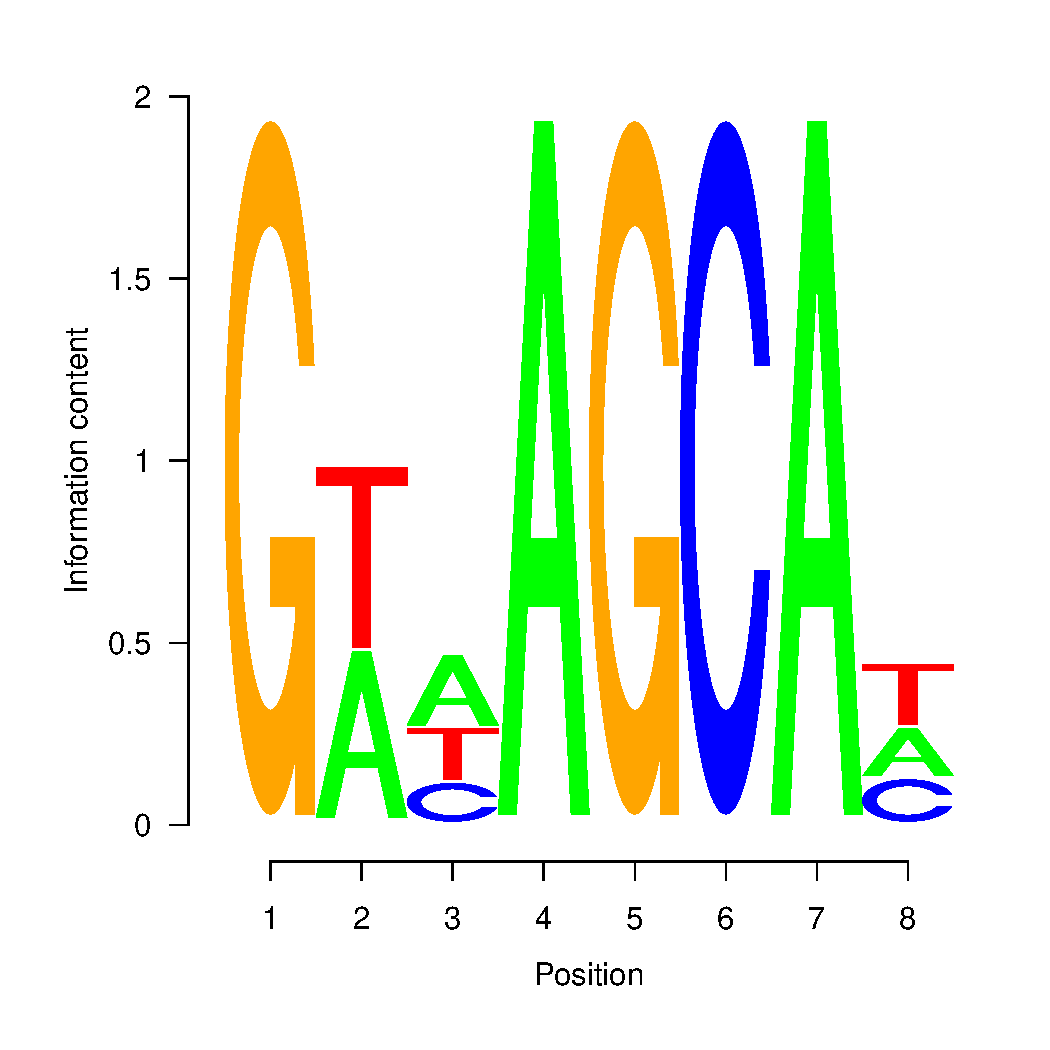
\includegraphics[width=9cm]{seqlogo.pdf}
   \caption{One of the motifs identified by \Rpackage{BCRANK}}
   \label{fig:seqlogo}
\end{figure}

\section{Version Information}
\begin{kframe}
\begin{alltt}
\hlkwd{toLatex}\hlstd{(}\hlkwd{sessionInfo}\hlstd{())}
\end{alltt}
\end{kframe}\begin{itemize}\raggedright
  \item R version 3.2.5 (2016-04-14), \verb|x86_64-pc-linux-gnu|
  \item Locale: \verb|LC_CTYPE=en_US.UTF-8|, \verb|LC_NUMERIC=C|, \verb|LC_TIME=en_US.UTF-8|, \verb|LC_COLLATE=en_US.UTF-8|, \verb|LC_MONETARY=en_US.UTF-8|, \verb|LC_MESSAGES=en_US.UTF-8|, \verb|LC_PAPER=en_US.UTF-8|, \verb|LC_NAME=C|, \verb|LC_ADDRESS=C|, \verb|LC_TELEPHONE=C|, \verb|LC_MEASUREMENT=en_US.UTF-8|, \verb|LC_IDENTIFICATION=C|
  \item Base packages: base, datasets, graphics, grDevices, methods, parallel,
    stats, stats4, utils
  \item Other packages: Biobase~2.30.0, BiocGenerics~0.16.1, BiocParallel~1.4.0,
    Biostrings~2.38.2, DBI~0.3.1, GenomeInfoDb~1.6.1, GenomicAlignments~1.6.1,
    GenomicRanges~1.22.1, IRanges~2.4.4, knitr~1.12, Rsamtools~1.22.0,
    RSQLite~1.0.0, S4Vectors~0.8.3, ShortRead~1.28.0, SummarizedExperiment~1.0.1,
    systemPipeR~1.4.8, XVector~0.10.0
  \item Loaded via a namespace (and not attached): annotate~1.48.0,
    AnnotationDbi~1.32.0, AnnotationForge~1.12.0, base64enc~0.1-3, BatchJobs~1.6,
    BBmisc~1.9, BiocStyle~1.8.0, biomaRt~2.26.1, bitops~1.0-6, brew~1.0-6,
    Category~2.36.0, checkmate~1.6.3, colorspace~1.2-6, digest~0.6.9, edgeR~3.12.0,
    evaluate~0.8, fail~1.3, formatR~1.2.1, futile.logger~1.4.1,
    futile.options~1.0.0, genefilter~1.52.0, GenomicFeatures~1.22.6, ggplot2~2.0.0,
    GO.db~3.2.2, GOstats~2.36.0, graph~1.48.0, grid~3.2.5, GSEABase~1.32.0,
    gtable~0.1.2, highr~0.5.1, hwriter~1.3.2, lambda.r~1.1.7, lattice~0.20-33,
    latticeExtra~0.6-26, limma~3.26.3, magrittr~1.5, Matrix~1.2-3, munsell~0.4.2,
    pheatmap~1.0.7, plyr~1.8.3, RBGL~1.46.0, RColorBrewer~1.1-2, Rcpp~0.12.3,
    RCurl~1.95-4.7, rjson~0.2.15, rtracklayer~1.30.1, scales~0.3.0, sendmailR~1.2-1,
    splines~3.2.5, stringi~1.0-1, stringr~1.0.0, survival~2.38-3, tools~3.2.5,
    XML~3.98-1.3, xtable~1.8-0, zlibbioc~1.16.0
\end{itemize}


\section{Funding}
This project was supported by funds from the National Institutes of Health (NIH) and the National Science Foundation (NSF).

\bibliography{bibtex}

\end{document}
